%!TEX root = ../thesis.tex
%*******************************************************************************
%****************************** Second Chapter *********************************
%*******************************************************************************

\chapter{Related work}

\ifpdf
\graphicspath{{Chapter2/Figs/Raster/}{Chapter2/Figs/PDF/}{Chapter2/Figs/}}
\else
\graphicspath{{Chapter2/Figs/Vector/}{Chapter2/Figs/}}
\fi

\section{Human behaviour modelling}
%%FR In generale, quando fai uno statement devi supportarlo con un riferimento. Non sei TU che dici queste cose, qui stai riportando le opinioni della comunità scientifica.

%%FR Non parli di methodi tipo SKNN, ma nei tuoi studi ti confronti con questi. Forse dovresti mettere qualcosa nello stato dell'arte.

\label{sec:human_behaviour_modelling}
In this thesis, with human behaviour we refer to the course of actions an individual or a group of individuals take in order to complete a task, like deciding which book to read under the beach umbrella or which restaurant to reserve for a family lunch. Therefore, we discuss here the highly complex cognitive process, characterizing Human-decision making, that leads to the decision to perform an action, e.g., choosing which book to read among several possible books (the full set of choices).

Decision-making is a study subject of many disciplines, like economy, psychology, philosophy and computer science. A decision maker is a human or more generally an intelligent agent, that has a reasoning mechanism that enables it to make choices. Typically, it is assumed that the agent is rational, i.e., the agent is self-interested and acts in order to maximise the incentives 
%%FR incentives or gain, reward. Incentivo e' una cosa particolare.
that it can obtain from its choices \cite{decisionmaking:Kahneman,rational:utility:def}. That said, in order to maximise its objective (the collection of incentives), the agent must know all the possible choices and the related incentives. 
%%FR In generale in DM si dice che le choices hanno degli outcome, in relazione ai possibili world states.
A way to model the human (agent) 
%%FR ora parli di uomini, prima parlavi di agenti. E' fatto di proposito?
behaviour is to define a measure that quantifies the consequences (how many incentives)
%%FR "how many incentives"??? Sono numerabili?
of the future agent's choices. 
%%FR non sono le azioni che sono future, penso, ma l'outcome.
That said, the utility tells us how much the agent is or is foreseen to be ``satisfied''. 
In order to compute the utility of the agent's choices a mathematical model is needed; it can be defined by an expert (e.g., a behavioural scientist) or inferred from the observations of an agent's (or group of agents) actions.

An expert that formulates the mathematical model that captures the underlying reasoning mechanism of an agent, acts according to this three steps: knowledge extraction; model formulation; model evaluation. The process of extracting the domain knowledge can be achieved by interviewing decision-makers in the domain under investigation. Then, it follows the mathematical formulation of the reasoning mechanism. Finally, the designed decision model can be assessed by observing the deviation of the decisions performed by humans and those that are the outputs of the model.

The second approach to decision-making modelling grounds on observational data of user (agent) choices (actions).
%%FR ora parli di "user". Sarebbe bene usare solo un termine in maniera uniforme e spiegare la prima volta
%% che lo usi a cosa ti riferisci.
Learning from data can exploit techniques developed by researchers and practitioners in the field of Machine Learning (ML). A ML model takes as input observational (behaviour) data and by leveraging statistics
%%FR Che statistics? Tecniche, principi .... 
predicts an agent's actions. In this thesis we model human decision-making in a data-driven fashion. 

\subsection{Machine Learning for human behaviour prediction}
In ML the need of domain knowledge is generally limited to the definition of the settings in which the decision-maker is acting. This is typically done by modelling the decision-maker as a vector, 
%%FR faccio difficolta' ad immaginare che SEMPRE in ML per modellare un decision maker si usa un vettore.
%% Chi lo ha detto? Devi mettere un riferimento. Secondo me tu stai facendo riferimento a degli approcci specifici.
%% Puoi essere piu' specifico?
which elements  represents meaningfully the characteristics of the decision scenario. For instance, if we want to build an agent that mimics the decision-making process of an individual that has to book an hotel for a work travel,
%%FR mi aspettavo che tu introducessi un decision tree, per esempio.
we should consider as the vector components, features such as the travel dates and the budget the decision maker is ready to pay for his stay. The numerical values that allows to identify the hotel the user will probably decide for can be computed in several ways; this ways of identifying a choice (solution) are grouped in these areas of ML.
%%FR Il vettore rappresenta i vincoli sul prodotto che deve essere scelto? Non mi e' chiaro come questo possa rappresentare quello che dici all'inizio "the settings in which the decision-maker is acting".
\newline


\noindent\textbf{Supervised learning} \cite{Russell:2009:AIM:1671238} models takes as input past user's choice observation data in order to approximate the user's decision making process. 
%%FR Io non parlerei di "process" perche' fa pensare ai passi di soluzione. Qui, in realtà stai solo dicendo che con questa tecnica si puo' modellare/prevedere la scelta, a partire da alcune informazioni che caratterizzano il problema decisionale.
Approximating the choices of a user is possible due to the presence of labels, that annotates the observed choice actions, in the training data. For instance, in the case of the previous hotel booking example, the training data can consist in the amount of money the user want to spend, check-in and check-out dates and the booked hotel. \newline
%ML models like decsion trees, NN adn SVM have been succesfully applied to human decision making.

\noindent\textbf{Unsupervised learning} \cite{unsupervised:Hinton1999} aims at discovering more about the data rather than approximating the user behaviour. Such models are employed when data cannot be labelled and there is the need to have a deeper insight about the underlying distribution or patterns in the data. For instance by applying clustering, we can identify specific groups of hotels' guests just by having their demographic information. Then, these groups can be further studied in order to gain more insight about their decision making process. \newline


\noindent\textbf{Reinforcement learning} \cite{sutton:1998} is the ML technique that frames DM closer to how a behavioural scientist or economist see real decision-making. In Reinforcement learning an individual 
%%FR ora lo chiami "individual".
(agent) is self-interested and acts with the intent to optimize an objective. 
%%FR objective function?
The environment in which the agent acts is unknown to it. The agent's choices are made in such a way that the cumulative reward it can obtain from its actions is maximised. The reward can be intended as the utility (or satisfaction) the agent gets by acting in a specific way. In a similar way to expert-driven behaviour modelling the reward an agent collect by its interaction with the environment is defined by an expert. By employing an RL agent it is possible to map states describing the decision environment to actions, 
%%FR non capisco cosa dici sopra. States e action sono cose distinte, un'action determina una transizione di stato.
learning in this way the policy, 
%%FR non e' chiaro come "learning in this way ..."
or even better an optimal policy, that tells the agent how it should act in order to maximise its cumulative reward given its current state.
When observations of human decisions are available then a policy (i.e., the human behaviour) can be learnt from the data by using Inverse Reinforcement Learning. 
%%FR devi enfatizzare la differenza con quanto detto sopra. Non e' chiara.

Applications of ML models in which human behaviour is the learning objective are, for instance: learning the health status of citizens from food purchases \cite{health:aiello:2019}; learning and predicting individual's lifetime expectation and health leveraging smokers behavioural data \cite{smokers:darden:2017}; learning planning strategies of herders \cite{ermon:2015}; learning user preferences about items (e.g., movies) by observing online users' behaviour in order to generate recommendations about items they will like to consume in the future \cite{RSdef:2015}.
%Human behaviour modelling and learning is a fundamental part of many application is computer science, like in social networks or recommender systems. 
In this thesis we focus on modelling user behaviour for applications to Recommender Systems.

\section{Recommender Systems}
\label{sec:recommender_system}
Recommender Systems (RSs) are software tools that aim at easing people 
decision making by delivering personalised suggestions about items to 
consume or actions to perform \cite{RSdef:2015}. 
Nowadays, RSs are key elements 
%%FR "elements" e' generico. Usa un termine piu' specifico.
placed at the core business of many companies in a variety of sectors, like tourism, e-commerce, video and music streaming.\footnote{Examples of companies that successfully employed RSs are: in the tourism domain, Booking.com, Expedia and Tripadvisor; in E-commerce, Amazon and Idealo; in the video and music industry, YouTube and Spotify.}
%%FR perche' usare una footnote?
The success of RSs in business applications is due to its dual function to serve both the company strategy and the end user's need as well. As reported in \cite{RSdef:2015} examples of these functions are, from the company perspective: increase the quantity of items sold; increase the user satisfaction; increase the fidelity of the user. Instead, the end user is supported to: find good items; find relevant items; help other users to find good/ relevant items.  

A RS in order to identify items that are suitable for a user needs to estimate the utility of the items in the system dataset. The typical assumption in RS is that the user wants to maximise the utility associated with an item. This is similar to what is presented in Section \ref{sec:human_behaviour_modelling}. In order to perform the computation of this utility a RS needs to process observation data about the user (past) behaviour, e.g., which are the items purchased by the user or what are the features that characterizes the purchased items. So, these observations may capture at different extent the information about the user actions (e.g., clicks or purchases) and the item information (e.g., description).

Given the user behaviour data a RS can employ different techniques to identify which items are relevant for a user.
%The two most popular approaches for recommendation generation are content-based \cite{contentbased:lops} and collaborative filtering (CF) \cite{cf:koren}. 

\subsection{Recommendation techniques}
A classification of the methods that have been devised and deployed to generate recommendations for a target user are here presented. \newline

\noindent\textbf{Content-based} RSs \cite{contentbased:lops} suggest items of interest based on an analysis of their features. For instance, a media recommender system 
exploits the features of the media content (such as topic, length or media 
type) and suggests items that have the features contained by media that 
the user has consumed or liked before. \newline

\noindent\textbf{Demographic} recommendations techniques \cite{demographic:RSdef} identify items to be suggested to a user by leveraging her demographic information. The motivation of this method is rooted in the idea that different type of user need different type of recommendations. For instance, a user of a Point of Interest RS may be suggested to visit the most popular places if she is a tourist, whereas in the case she is a local the recommendation can be to visit more niche places.\newline

\noindent\textbf{Knowledge-Based} recommendations \cite{kb:RSdef} are generated by relying on rules that establish how certain item features satisfy the user needs and preferences. From the human behaviour modelling perspective such systems are expert-driven. The system designer infer from the domain knowledge a mathematical function that computes the similarity of the user needs and the possible recommendations. \newline

\noindent\textbf{Collaborative Filtering} \cite{cf:koren} identifies items to recommend to the target user by exploiting only information pertaining to her actions (consumed items) and those of similar users. 
%%FR Ad essere precisi sono item che l'utente ha valutato
Users are considered similar if they acts similarly, e.g., they rate higher a specific item and lower another item. Collaborative Filtering is based on two types of user behaviour data: explicit feedback data, like ratings and likes, or implicit feedback data, like clicks on a webpage.  While explicit feedback is usually in a binary scale (i.e. like or dislike) or a likert-scale (star ratings), implicit feedback \cite{Hu2008,Pan2008,gurabnov:2016} recommendation techniques exploit observations of users' actions performed on the items. For instance, a RS, in order to suggest an internet video, could exploit data about browsing behaviours while watching videos, e.g., the fact that certain videos are skipped or partially seen.\newline
%When more approaches are combined together to overcome limitations of single solutions, we speak about hybrid approaches \cite{hybrid}.

\noindent\textbf{Hybrid} RSs \cite{hybrid:RSdef} combine two or more of the presented recommendation strategies in order to improve the quality of the suggested items avoiding the pitfalls of a specific strategy by leveraging the benefits of another RS technique. For instance, the inability of Collaborative Filtering methods to compute the utility of an item if user-item interactions are absent in the observation data, can be overcome by exploiting the capability of Content-based methods to harness the descriptive features of the item to identify items with the same (or a subset) of features that the user (or users) consumed before.\newline


Since the motivations behind the choices of a user may depend on external factors, that defines the decision context of the user, e.g., the time or the location dimensions in which the user is placed, Context-aware RS (CARS) have been proposed. CARSs tries to improve recommendations by considering the user preferences about items and by modelling the context in which an item has been consumed in order to predict which item will be more likely consumed by users that are in a given context \cite{adomavicius:2011}. CARSs have been used in various application domains like news, movies and tourism \cite{lommatzsch:news:2017, adomavicius:movie:2005, braunhofer:sts:2015} and several context modelling techniques have been proposed \cite{baltrunas:2012,braunhofer:2017}. \newline


%All the presented recommendations models learn to predict the item utility for a target user by exploiting the observed past user-item interactions. According to our knowledge, those items that the user explicitly ignores, or the specific order in which the user acts on them, is a valuable information that has not been fully exploited yet. We think that these aspects are a valuable source of information to model, at first, the action selection policy users follow when choosing items to consume, especially in sequential decision making processes. Then, to model the user preferences about certain items. Hence, we can better model the human behaviour of RSs users and then harness it to generate more useful recommendations. 
%For instance, let us consider observations of a tourist that is interested in museums and is visiting a new city. The tourist went first to a cafeteria, then visited a local art museum to end up in a book shop even if in the surroundings there are several museums. This pattern could indicate us that the user action selection policy can be of visiting museums, but not in a row.
In this thesis in order to learn better users' action selection policies and preferences, we aim at finding a context-model that can be leveraged by recommendations techniques that generate effective sequences of recommendations to a user.

\subsection{Sequential recommendations}
\label{sec:sequentialrecommendation}
Most of the approaches exploited in RSs implicitly assume that the consumption of 
goods and their evaluations are independent from the order in which the items have been accessed. 
%%FR consumed? Perche' ora usi il termine "accessed", sembra che questa distinzione abbia senso per quello che vuoi dire.
For instance, content-based and collaborative based techniques do not exploit the users's item evaluation order to build their predictive models.
In some cases, rather than predicting a set of items that could be relevant for a user, the goal is to identify items that could be consumed immediately after a specific item. For instance, during a visit in the city of Bolzano (Italy) what can be recommended to a tourist that visited, at first, Walther square and, then, an exhibition in Museion, that are two very close but different venues?
In order to address this type of questions, the sequential aspect of item consumption 
has been studied in the context of personalisation by proposing pattern-discovery approaches in different domains: web \cite{mobasher:2002}, music \cite{hariri2012, jannach2017}, travel \cite{zhang:seq:travel:2014,flikr_tourism_RS:muntean:2015,palumbo:2017} and cultural heritage \cite{hashemi:2017}. 
%These techniques exploit observations of user actions in order to discover patterns to be used to predict sequences of actions users can perform. For instance, the sequences of songs listened by a user could be used to predict which songs can be played next.

Alternatively, Reinforcement Learning techniques have been employed in order to design a RS that considers the items' consumption order. In \cite{shani:RS:MDP:2005,moling:rl:seq} were computed optimal decision making policies to offer adapted content as a sequence of items to users, whereas in \cite{mahmood:seq:rl:2009} Reinforcement Learning was used to compute the optimal interaction policy of a conversational recommender whose suggestions were generated with case-based reasoning.

In the first approach, common patterns in users' behaviour logs (users' choices) are identified and a predictive model of the next user choice is learnt. In the second one, recommendations are generated by exploiting an optimal choice model (policy) that is learnt from the utility (reward) that the system is supposed to obtain by showing certain information to the user in response to the user's requests. A common feature of both approaches is that the recommended items are the predicted next choices of the target user. Moreover, the first approach can only suggest items that have been already observed, i.e., it suffers from the new item problem, whereas the second one assumes that the system knows the utility the user gets from her actions, while in practice users rarely provide explicit feedback (e.g., ratings). One major drawback of these techniques is that they tend to generate recommendations that lack novelty and that therefore tend to be not interesting for the user \cite{vargas2011}. \newline

In this thesis, in order to not suggest uninteresting items to users and to deal with situations in which users' explicit feedback is scarce, we propose a recommendation technique that harnesses a generalised user behavioural model that is learnt via Inverse Reinforcement Learning (IRL) by observing a group of users (cluster) ``similar'' to the target one.

\section{Inverse Reinforcement Learning}

To fulfil the need of learning an explainable user behavioural model from user behaviour data, imitation learning is a viable solution. It is typically addressed by solving Markov Decision Problems (MDP) via Inverse Reinforcement Learning (IRL)\cite{ng:2000}.
A MDP is defined by a tuple $(S,A,T,r,\gamma)$. $S$ is a finite set of states (e.g., visit to a location). $A$ is a finite set of actions (e.g., moving to a location). $T$ is a finite set of probabilities $T(s'| s, a)$, to make a transition from state $s$ to $s'$ when action $a$ is performed.
The function $r: S \rightarrow \mathbb{R}$ models the reward a user obtains from acting in a certain way (being in a state). This function is supposed to be {\it unknown} and must be learnt.


Given a demonstrated behaviour (e.g., user actions sequences), IRL models solve the target MDP by computing the reward function that makes the behaviour induced by the optimal policy for that reward (the learning objective) close to the demonstrated behaviour.
Despite the fact that the reward is learnt from behaviour observation, the induced policy may not uniquely identified. It means that an IRL problem has many solutions. In order to overcome this problem several algorithmic strategies has been proven to identify a solution that justifies the observed behaviour. In \cite{ng:2000} the authors suggest to introduce a margin to a linear programming formulation of the IRL problem, such that the difference between the (learnt) reward obtained from a policy and the reward of other policies is maximised. In \cite{maxentirl} the reward function is sought by matching state features in the observation data. Maximum-entropy is used to identify actions probabilities that lead to a reward that supports the observed actions.
In \cite{vro:litt:2011} the identification of a solution that supports the observations is identified by combining maximum likelihood estimation with a gradient method.
%The reward is typically computed by a function that maps the state of an agent, i.e., a vector which elements are features representing, e.g., its decision context or the characteristic of the consumed item, to real values.
%%FR Mi domando se poi tu non debba spiegare un po' meglio gli algoirtmi che hai usato. Lo fai qui o nella sezione in cui descrivi le tue tecniche?



\subsection{Applications of IRL methods}.
In \cite{maxentirl} the authors developed an IRL approach based on the principle of maximum entropy that is applied in the scenario of road navigation. The approach is based on a probabilistic method that identifies a choice distribution over decision sequences (i.e., driving decisions) that matches the reward obtained by the demonstrated behaviour. This technique is useful to model route preferences as well as to infer destinations based on partial trajectories.
In \cite{irl:pedestrian} the author applies maximum entropy IRL in order to learn pedestrian behaviour from observed traces. The learnt behavioural model is used to generate synthetic trajectories at the city level in order to conduct simulations in planning tools. The IRL-based solution outperforms a popular baseline used in the sector of mobility and transportation to generate users' movements.
In \cite{ermon:2015} the authors propose an IRL-based solution to the problem of learning a user behaviour at scale. The application scenario is migratory pastoralism, where learning involves spatio-temporal preferences and the target reward function represents the net income of the economic activity. Similarly, in \cite{Kennan2011} it is proposed a method for computing the reward humans get from their movements decisions. The paper presents a tractable econometric model of optimal migration, focusing on expected income as the main economic influence on migration. The model covers optimal sequences of location decisions and allows for many alternative location choices. All these works, focus on designing a choice model without studying their application to RSs. 
%The formulation of an IRL problem is argument of Chapter \ref{cha:behaviour_learning}.

Leveraging IRL for behaviour learning allows not only to learn users' behaviour from implicit or explicit feedback data, taking into consideration the sequential nature of the item consumption, but also enables the to predict users' preferences about items that are unknown for them. This is possible thanks to the ability of IRL models to generalize over a set of features describing the items. 

\section{Collecting human behaviour data}
In the era of Ubiquitous computing, where people are constantly connected to the internet through their mobile devices, user behaviour data are generated incredibly fast. 
Generated data can capture the user's interactions in the virtual world, e.g., clicks on web pages, as well as the user interactions in the physical world, e.g., the user user location.
In this thesis we use the term ``online behaviour'' to refer to the user interactions in the virtual sphere, whereas ``offline behaviour'' refers to the user actions in the physical world.

\textbf{Online user's behaviour} data are essentially the source of information used as input in RSs (Section \ref{sec:recommender_system}). Summarizing, the records of a user actions on the web are distinguished in: explicit actions (feedback), like ratings given by the user to movies on a streaming platforms that are expressing the utility that the user perceive to get from the item, and implicit feedback, like the click on the skip button of a media player that can be interpreted as a sign that the user didn't complete the consumption of the media content because she is not happy with it. Similarly, users' explicit and implicit actions/feedback can be identified in the user's offline behaviour. 

\textbf{Offline user's behaviour} consist of records of individual's physical actions like moving from a location to another location or picking an item from the shelf, as well as paying with a credit card in a shop. In general, we can say that offline behaviour is a locational data source. 
%%FR fai un riferimento a chi ha usoto questo termine; da dove deriva.
Here we list the most used types of offline behaviour data.
%%FR nei RSs? o in generale? In che cosa?

\begin{itemize}
	\item \textbf{Call Details Records} (CDRs) are data collected by cellular network operators that keep records of mobile communications. A mobile cell, covers a portion of a geographical area with a radio-frequency, with a radius that goes from 1 to 30 kilometers, and allows to transmit mobile signals, e.g., phone calls. 
	%%FR non direi che una telefonata e' un signal. Si usa questo termine per indicare il fenomeno fisico. Una telefonata trasporta informazioni. Un'onda elettromagnetica trasporta un segnale in cui informazione e' stata codificata.
	Cells are positioned close to each other in order to cover large areas and allow communication while the user of the network, e.g., the phone caller, is moving. CDRs data offer a compromise between the space (location) and time dimension of a user. 
	%%FR Non capisco cosa intendi per "compromise" in questo caso.
	Learning human behaviour from CDRs data has been successfully done in the context of human activity recognition for the design of activity-based travel demand models \cite{cdr:urban:humanActivita:HMM:Feygin:2018}. The authors in \cite{cdr:urban:jacobsMetrics:quercia:2016} exploits CDRs data in combination with external information sources, like, census, land-use and social-network data in order to enable urban planners and sociologist to measure with an automated tool the ``vitality'' metrics of a city.
	
	\item \textbf{GPS} data provides fine-grained location data of moving objects, e.g., people, cars and cattle, in both the space and time dimension. The typical format consist of a pair of latitude and longitude coordinates annotated with a timestamp and the accuracy of the measure. Errors on the recorded locations are in the range of few meters and each location update can be recorded even at the scale of seconds.
	Processing GPS datasets in order to identify precious insight about the behaviour of moving objects has been extensively studied in trajectory data mining. In \cite{gps:geolife} the authors proposes techniques for travel recommendations base on stay point detection of people's raw GPS data. GPS data are processed to identify clusters of records that, thanks to a timestamp annotation, allow to identify candidates locations where the user performed some activity. In transportation applications, rather than having the information about stay points of individuals, is important to understand which are the road segments traversed by the user and her direction. In \cite{gps:mapmatching:HMM} is proposed a map-matching model that can provide an high accuracy traversing behaviour of a moving object. By starting from raw GPS traces the model considers transition probabilities and the topology of the road network and identifies the actual segments traversed by the user.
	
	
	\item \textbf{Location Based Social Network} (LBSN) data is a rich resource that combines exact location data annotated with user feedback, like, ratings, reviews or opinions about the location. Nowadays, many deployed online systems are LBSN, these are, for instance, Foursquare (location and opinion sharing) and Waze (navigation). Given the richness of their records, LBSNs have been extensively used to model and predict human behaviour. In \cite{lbsn:clusteringUsers,lbsn:gentrification} LBSN data are extensively used to analyse and explain social aspects at the urban level, like, understanding how diverse groups of citizens interacts with the surrounding space.
	The deep level of understanding about the places where a user spent time and her opinion of them comes at the cost of having very sparse data. LBSNs users have to explicitly insert data records in the system and therefore, as it usually happens in information systems, the user feedback is rather scarce. This makes the usage of check-in data for sequential decision-making inference, like deciding which route or the next location to visit, more difficult than GPS data. 
	
	%\item \textbf{Mobile Sensors} fff
	
	\item \textbf{Internet of Things} (IoT) is a dynamic and global adaptive network assisted by an intelligence that coordinates the communication between the connected 
	devices, the so called \emph{things}, in order to achieve a goal \cite{iotdef:li,li:zhao:2015,atzori:morabito:2011}.
	IoT relies on the following technologies: radio-frequency identification (RFID), Near Field Communication (NFC), low energy wireless communication (i.e. beacon) and Wireless 
	Sensor Networks (WSN) which are networks that connects these sensors via wireless communication.
	IoT enables to collect diverse type of feedback from humans. For instance, by placing IoT devices in an environment it is possible to respond to users' actions in real time as well as collecting data about their behaviour \cite{iot:notifications, iot-sensor-healthcare, petrelli2013integrating}. Human-IoT interactions can be enriched with location data, e.g., using the network or GPS on the user's mobile or by using the IoT device location. Hence, this type of data can provide both implicit and explicit information about the user activities that can be leveraged to analyse and learn human behaviour. 
\end{itemize}

In order to collect users' actions data and contextual information to learn users' preferences and behaviour, in this thesis we discuss a learning solution that exploits and combines as input sources: users' GPS traces; users-IoT interactions in IoT augmented spaces; external web repositories like LBSNs. Due to the nature of the data, observations of actions for which the user's reward is unknown, we base the learning solution on IRL.
The objective of designing RS technologies that harness the users' learnt behaviour is achieved by: setting up a proper context-model that can capture the decision situation of a user; identifying behaviour and preference patterns of the users by means of unsupervised learning, i.e., clustering; exploiting, as in Content-based RSs, the information about the user's consumed items, e.g., visited places.


%If you have trouble viewing this document contact Krishna at: \href{mailto:kks32@cam.ac.uk}{kks32@cam.ac.uk} or raise an issue at \url{https://github.com/kks32/phd-thesis-template/}

\begin{comment}
\begin{figure}[htbp!] 
\centering    
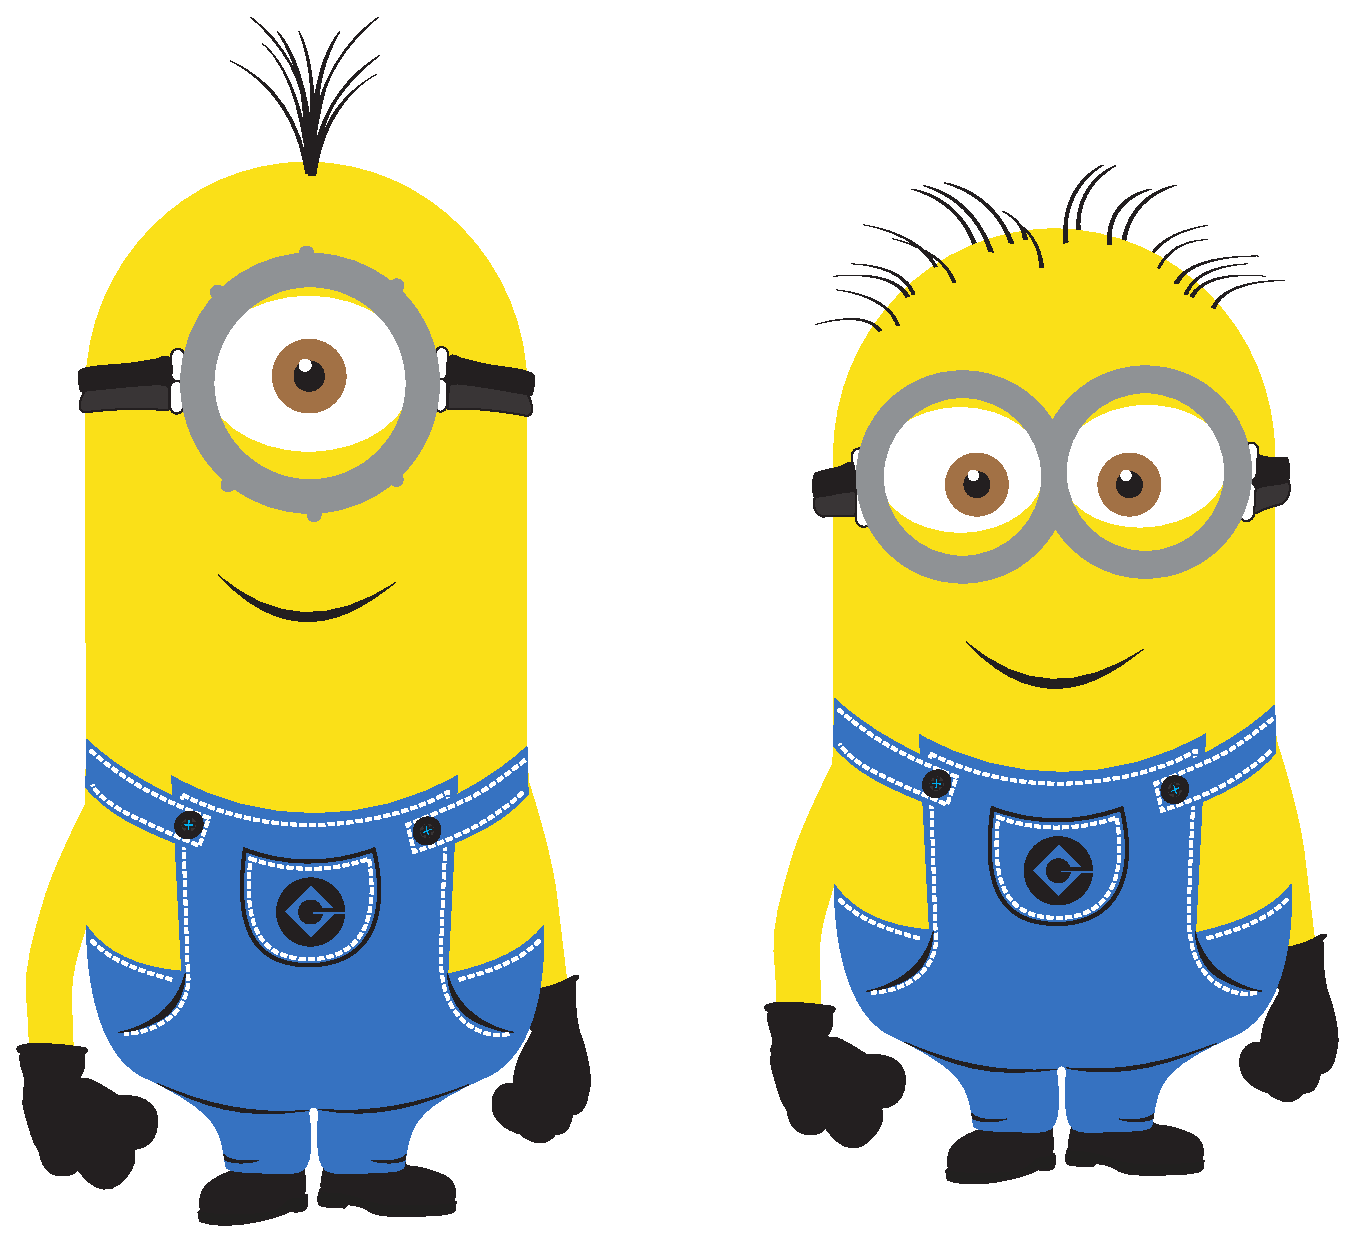
\includegraphics[width=1.0\textwidth]{minion}
\caption[Minion]{This is just a long figure caption for the minion in Despicable Me from Pixar}
\label{fig:minion}
\end{figure}
\end{comment}


\begin{comment}
\section*{Enumeration}
Lorem ipsum dolor sit amet, consectetur adipiscing elit. Sed vitae laoreet lectus. Donec lacus quam, malesuada ut erat vel, consectetur eleifend tellus.
\begin{enumerate}
\item The first topic is dull
\item The second topic is duller
\begin{enumerate}
\item The first subtopic is silly
\item The second subtopic is stupid
\end{enumerate}
\item The third topic is the dullest
\end{enumerate}

Itemize.

\section*{Itemize}
\begin{itemize}
\item The first topic is dull
\item The second topic is duller
\begin{itemize}
\item The first subtopic is silly
\item The second subtopic is stupid
\end{itemize}
\item The third topic is the dullest
\end{itemize}

Description

\section*{Description}
\begin{description}
\item[The first topic] is dull
\item[The second topic] is duller
\begin{description}
\item[The first subtopic] is silly
\item[The second subtopic] is stupid
\end{description}
\item[The third topic] is the dullest
\end{description}


\clearpage

\tochide\section{Hidden section}
\textbf{Lorem ipsum dolor sit amet}, \textit{consectetur adipiscing elit}. In magna nisi, aliquam id blandit id, congue ac est. Fusce porta consequat leo. Proin feugiat at felis vel consectetur. Ut tempus ipsum sit amet congue posuere. Nulla varius rutrum quam. Donec sed purus luctus, faucibus velit id, ultrices sapien. Cras diam purus, tincidunt eget tristique ut, egestas quis nulla. Curabitur vel iaculis lectus. Nunc nulla urna, ultrices et eleifend in, accumsan ut erat. In ut ante leo. Aenean a lacinia nisl, sit amet ullamcorper dolor. Maecenas blandit, tortor ut scelerisque congue, velit diam volutpat metus, sed vestibulum eros justo ut nulla. Etiam nec ipsum non enim luctus porta in in massa. Cras arcu urna, malesuada ut tellus ut, pellentesque mollis risus.Morbi vel tortor imperdiet arcu auctor mattis sit amet eu nisi. Nulla gravida urna vel nisl egestas varius. Aliquam posuere ante quis malesuada dignissim. Mauris ultrices tristique eros, a dignissim nisl iaculis nec. Praesent dapibus tincidunt mauris nec tempor. Curabitur et consequat nisi. Quisque viverra egestas risus, ut sodales enim blandit at. Mauris quis odio nulla. Cras euismod turpis magna, in facilisis diam congue non. Mauris faucibus nisl a orci dictum, et tempus mi cursus.

Etiam elementum tristique lacus, sit amet eleifend nibh eleifend sed \footnote{My footnote goes blah blah blah! \dots}. Maecenas dapibu augue ut urna malesuada, non tempor nibh mollis. Donec sed sem sollicitudin, convallis velit aliquam, tincidunt diam. In eu venenatis lorem. Aliquam non augue porttitor tellus faucibus porta et nec ante. Proin sodales, libero vitae commodo sodales, dolor nisi cursus magna, non tincidunt ipsum nibh eget purus. Nam rutrum tincidunt arcu, tincidunt vulputate mi sagittis id. Proin et nisi nec orci tincidunt auctor et porta elit. Praesent eu dolor ac magna cursus euismod. Integer non dictum nunc.


\begin{landscape}

\section*{Subplots}
I can cite Wall-E (see Fig.~\ref{fig:WallE}) and Minions in despicable me (Fig.~\ref{fig:Minnion}) or I can cite the whole figure as Fig.~\ref{fig:animations}


\begin{figure}
  \centering
  \begin{subfigure}[b]{0.3\textwidth}
    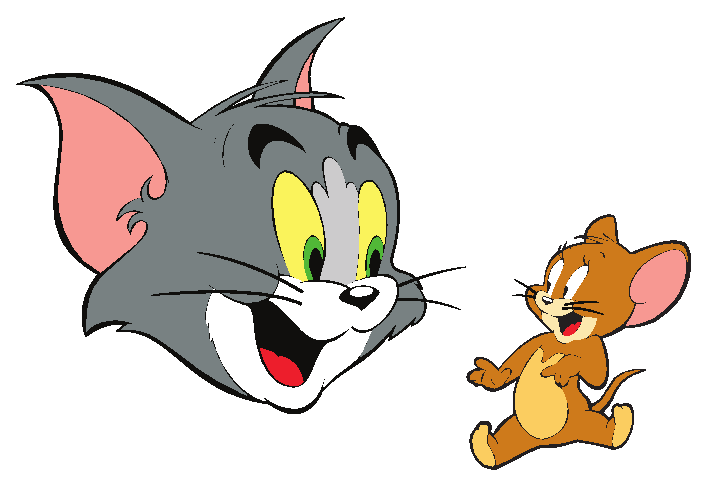
\includegraphics[width=\textwidth]{TomandJerry}
    \caption{Tom and Jerry}
    \label{fig:TomJerry}   
  \end{subfigure}             
  \begin{subfigure}[b]{0.3\textwidth}
    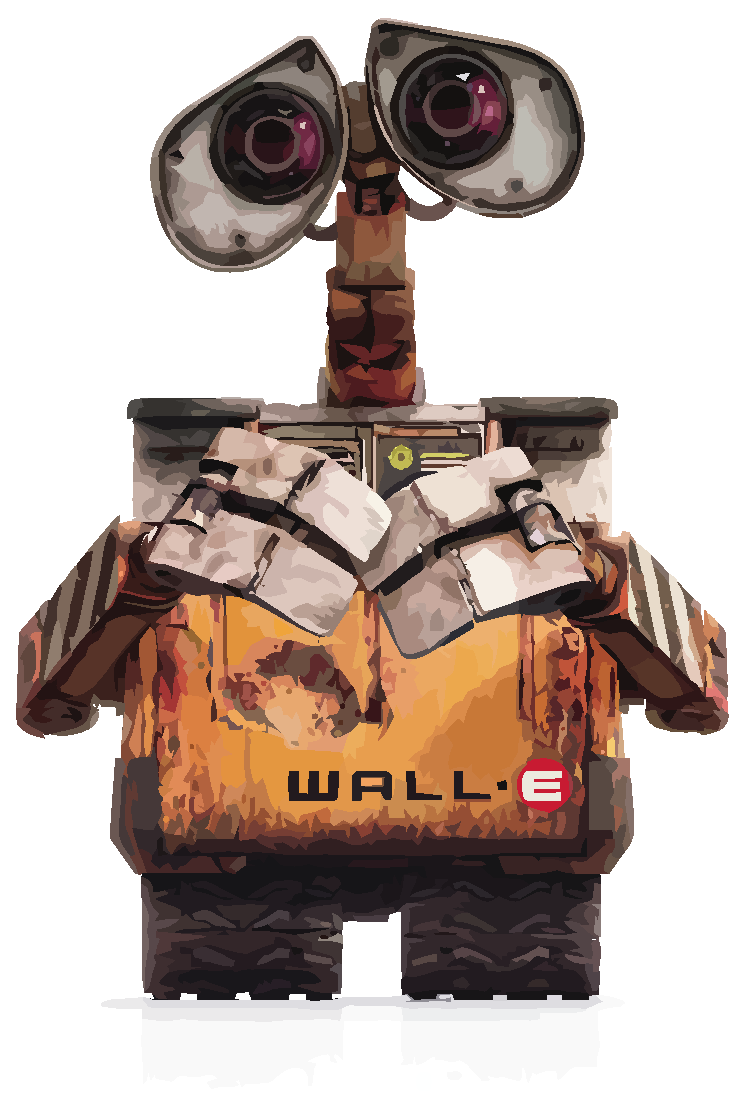
\includegraphics[width=\textwidth]{WallE}
    \caption{Wall-E}
    \label{fig:WallE}
  \end{subfigure}             
  \begin{subfigure}[b]{0.3\textwidth}
    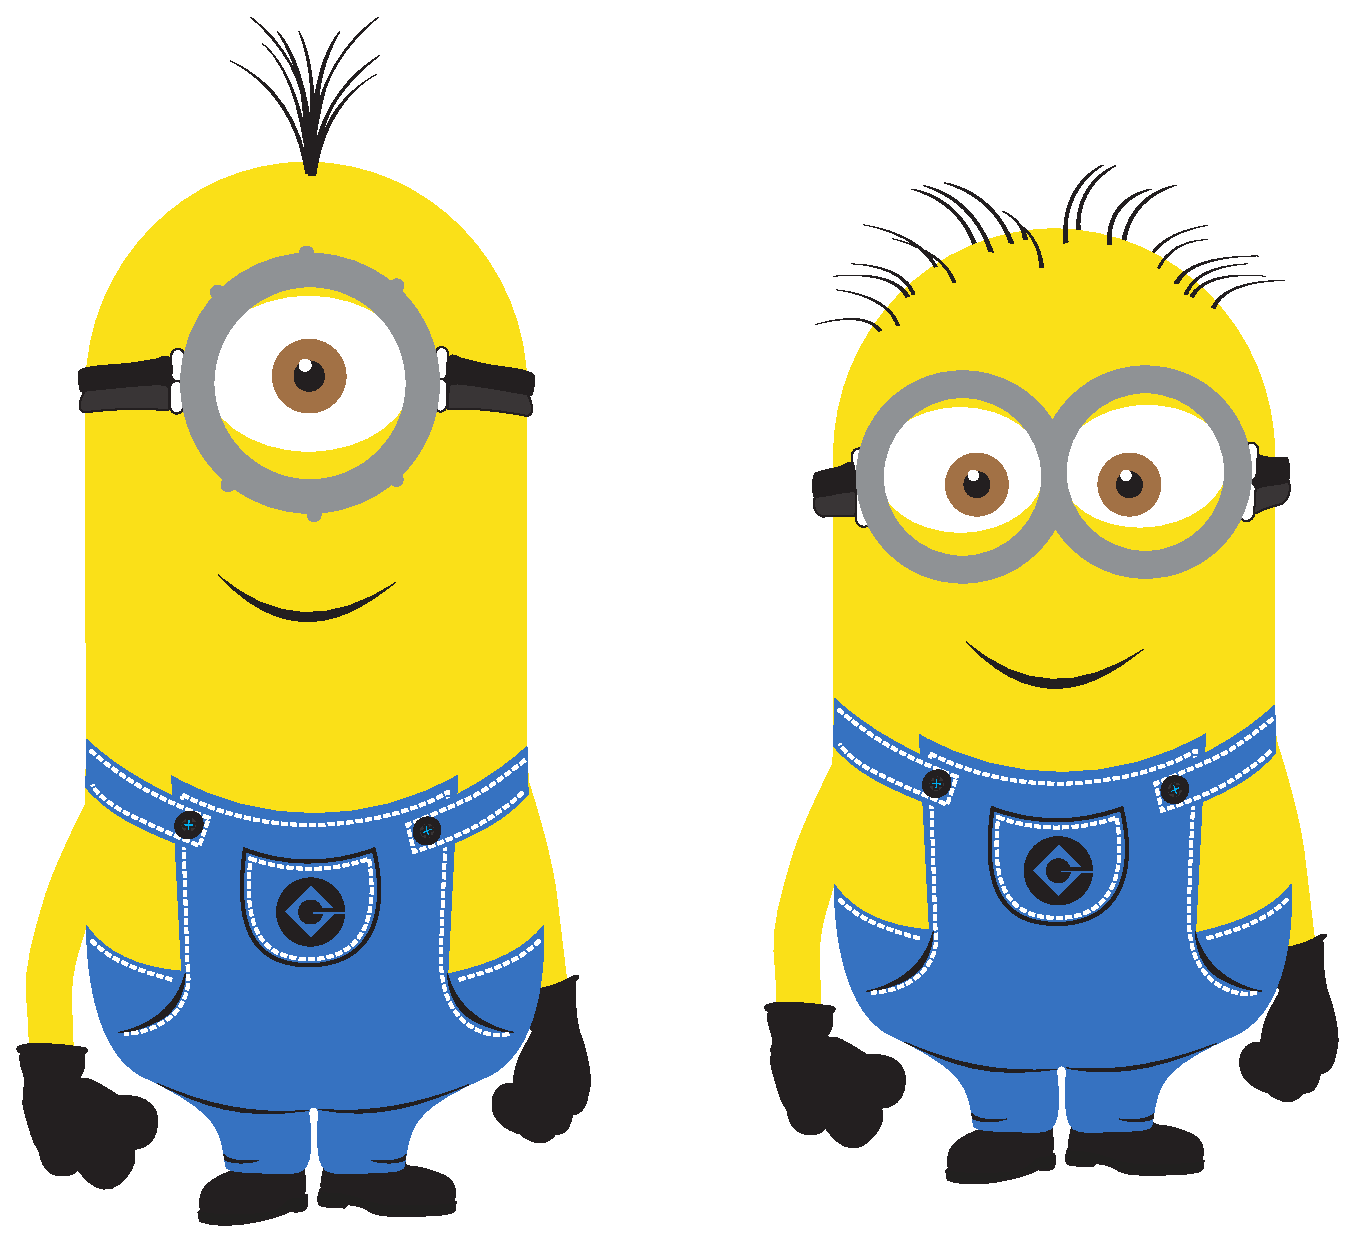
\includegraphics[width=\textwidth]{minion}
    \caption{Minions}
    \label{fig:Minnion}
  \end{subfigure}
  \caption{Best Animations}
  \label{fig:animations}
\end{figure}


\end{landscape}
\end{comment}